\documentclass[11pt,aspectratio=43,ignorenonframetext,t]{beamer}

% Presentation settings
\mode<presentation>{
  \usetheme[framenumber,titleframestart=1]{UoM_alex}
  \usefonttheme{professionalfonts} % using non standard fonts for beamer
  \usefonttheme{serif}             % set font to Arial
  \usepackage{fontspec}
  \setmainfont[Ligatures=TeX]{Arial}
}

% Handout settings
\mode<article>{
  \usepackage{fullpage}                  % use full page
  \usepackage{fontspec}                  % set font to Arial
    \setmainfont[Ligatures=TeX]{Arial}
  \setlength{\parskip}{1.5\baselineskip} % correct beamer line spacings
  \setlength{\parindent}{0cm}
  \usepackage{enumitem}
    \setlist[itemize]{topsep=0pt}
  \definecolor{uomlinkblue}{HTML}{0071BC}
}


% Packages

% Configurando layout para mostrar codigos C++
\usepackage{listings}
\lstset{
  language=Java,
  basicstyle=\fontsize{8}{10}\ttfamily, 
  keywordstyle=\color{blue}, 
  stringstyle=\color{orange}, 
  commentstyle=\color{gray}, 
  extendedchars=true, 
  showspaces=false, 
  showstringspaces=false, 
  numbers=left,
  numberstyle=\tiny,
  breaklines=true, 
  backgroundcolor=\color{blue!7},
  breakautoindent=true, 
  captionpos=b,
  xleftmargin=0pt,
}

\usepackage{graphicx}  % for graphics files
\usepackage{amsmath}   % assumes amsmath package installed
  \allowdisplaybreaks[1] % allow eqnarrays to break across pages
\usepackage{amssymb}   % assumes amsmath package installed 
\usepackage{hyperref} % add hyperlinks to document. Settings are for accessiblity
  \hypersetup{
    colorlinks=true,
    linkcolor=uomlinkblue,
    filecolor=uomlinkblue,      
    urlcolor=uomlinkblue,
	pdflang={en-GB},
}
\usepackage[document]{ragged2e} % left aligned text for accessibility
% experimental - does fundamentally work, if with quite a bit of effort
%\usepackage{axessibility} % LaTeX readable equations for accessibility
%  \tagpdfsetup{tabsorder=structure,uncompress,activate-all,interwordspace=true}
%  \pdfextension catalog{/Lang (en-GB)}
%  \RequirePackage{luacode}
%  \directlua{require("axessibility.lua")}
\usepackage{unicode-math} % unicode maths for accessibility
\usepackage{pdfcomment} % for alt text for accessibility
\usepackage{rotating}  % allow portrait figures and tables
\usepackage{subfigure} % allow matrices of figures
\usepackage{float}     % allows H option on floats to force here placement
\usepackage{multirow}  % allows merging of rows in tables
\usepackage{tabularx}  % allows fixed width tables
\usepackage{ctable}    % modifies \hline for use in table
\usepackage{bm}        % allow bold fonts in equations
\usepackage{pgf}       % allow graphics manipulation
\usepackage{media9}    % allow interactive flash files to be embedded
  \addmediapath{../media}
\usepackage{etoolbox}
  \makeatletter \preto{\@verbatim}{\topsep=0pt \partopsep=0pt} \makeatother  
  
% Custom commands
\newcommand{\matlab}{\emph{\sc{Matlab}}}
\newcommand{\maple}{\emph{\sc{Maple}}}
\newcommand{\simulink}{\emph{\sc{Simulink}}}
\newcommand{\dc}{d.c.}
\newcommand{\ac}{a.c.}
\newcommand{\rms}{RMS}
\newcommand{\wgn}{{\tt wgn}}
\newcommand{\sus}[1]{$^{\mbox{\scriptsize #1}}$}
\newcommand{\sub}[1]{$_{\mbox{\scriptsize #1}}$}
\newcommand{\chap}[1]{Chapter~\ref{#1}}
\newcommand{\sect}[1]{Section~\ref{#1}}
\newcommand{\fig}[1]{Fig.~\ref{#1}}
\newcommand{\tab}[1]{Table~\ref{#1}}
\newcommand{\equ}[1]{(\ref{#1})}
\newcommand{\appx}[1]{Appendix~\ref{#1}}
\newcommand{\degree}{\ensuremath{^\circ}}
\newcommand{\Vrms}{Vrms}
\newcommand{\Vpp}{V\sub{pp}}
\newcommand{\otoprule}{\midrule[\heavyrulewidth]}         
\newcolumntype{Z}{>{\centering\arraybackslash}X}  % tabularx centered columns 
\makeatletter \DeclareRobustCommand{\em}{\@nomath\em \if b\expandafter\@car\f@series\@nil \normalfont \else \bfseries \fi} \makeatother
\newcounter{example_number} % keep track of the example questions



%%%%%%%%%%%%%%%%%% FRONT MATTER %%%%%%%%%%%%%%%%%%
\title{Desenvolvimento de Software}
\subtitle{Aula 16 - Classes e métodods Abstratos}
\author{Prof. Me. Juliana Costa-Silva}

\begin{document}

\maketitle
%%%%%%%%%%%%%%%%%% TITLE SLIDE %%%%%%%%%%%%%%%%%%
\mode<presentation>{ \frame{\titlepage \label{slide:a}}} 
%\begin{figure}[!ht] 
%\fbox{\includeslide[width=\textwidth]{slide:a}} \end{figure}

%------------------------------------------------------------------------
\mode<presentation>{
\begin{frame}
\frametitle{Na aula de hoje...} 
\tableofcontents 
\end{frame}
}

\section{Introdução}
\begin{frame}{Na última aula...}
 \begin{itemize}
  \item Correção da prova
  \item Revisão de polimorfismo
  \item Atividade 
 \end{itemize}
\end{frame}
%-------------------------------------------------------
%----------------------------------------------------------------
\section{Introdução}
\begin{frame}{Classes Abstratas}{Conceito}
  Quando pensamos em um tipo de classe, logo pensamos em programas que criam objetos desse tipo.\\
As vezes é útil criar classes (chamadas \textbf{Abstratas}), para as 
quais você nunca pretende criar objetos.\\

\end{frame}
%----------------------------------------------------------------------------
\begin{frame}{Classes Abstratas}{Conceito}
  \begin{block}{Super Classes Abstratas}
    \begin{itemize}
     \item Utilizadas apenas para instanciar objetos, em hierarquias de 
herança, por isso chamadas \textbf{superclasses abstratas}.
      \item Não podem ser Utilizadas para instanciar objetos , por que como 
veremos mais adiante, classes abstratas são incompletas.
      \item As subclasses devem declarar as ``partes ausentes'' para que se 
tornem classes ``concretas''.
      \item Somente a partir de classes concretas você pode instanciar objetos.
    \end{itemize}

  \end{block}
  \textcolor{purple}{Em que momento isso pode ser útil?}
\end{frame}
%----------------------------------------------------------------------------
\begin{frame}{Classes Abstratas}{Finalidade}
  \begin{block}{Super Classes Abstratas}
    \begin{itemize}
     \item Utilizadas apenas para instanciar objetos, em hierarquias de 
herança, por isso chamadas \textbf{superclasses abstratas}.
      \item Não podem ser Utilizadas para instanciar objetos , por que como 
veremos mais adiante, classes abstratas são incompletas.
      \item As subclasses devem declarar as ``partes ausentes'' para que se 
tornem classes ``concretas''.
      \item Somente a partir de \textbf{classes 
concretas\tiny{\footnotemark[1]}} você pode instanciar objetos.
    \end{itemize}
  \end{block}
  \tiny{\footnote{Classes concretas, são classes que permitem a instanciação de 
      objetos.}}
\end{frame}
%-------------------------------------------------------------------
\section{Classes e métodos abstratos}
\begin{frame}{Classes e Métodos abstratos}{Exemplo}
  Para criar uma classe abstrata declaramos a classe com a palavra chave 
  \textcolor{purple}{abstract}.
  \begin{itemize}
   \item Uma classe abstrata normalmente tem um ou mais métodos abstratos
  \end{itemize}

\end{frame}
%----------------------------------------------------------------------------
\begin{frame}{Forma2D.java}
  Crie a classe abstrata Forma2D
 \small{ 
\lstinputlisting[linerange={2-17}]{./cod/aula16/Forma2D.java}}
\end{frame}
%----------------------------------------------------------------------------
\begin{frame}{Forma2D.java - Continuação}
 \small{ 
\lstinputlisting[linerange={22-38}]{./cod/aula16/Forma2D.java}}
\end{frame}
%----------------------------------------------------------------------------
\begin{frame}{Forma2D.java}
  Crie o método abstrato area.
 \small{ 
\lstinputlisting[linerange={20-20}]{./cod/aula16/Forma2D.java}}
\vspace{0.5cm}

\textbf{Toda \textcolor{purple}{subclasse} de Forma2D obrigatoriamente deverá 
implementar o método: double area()}.\\
A declaração de métodos abstratos só é permitida em classes abstratas.\\

\end{frame}
%----------------------------------------------------------------------------
\begin{frame}{Triangulo.java}
  Crie a subclasse de Forma2D: Triangulo
\small{\lstinputlisting[linerange={2-14}]{./cod/aula16/Triangulo.java}}
\end{frame}
%---------------------------------------------------
\begin{frame}{Triangulo.java}
  \textcolor{purple}{Erro!?} 
  Toda subclasse de uma classe abstrata deve 
implementar seus métodos abstratos, nesse caso area().\\
\small{
  \lstinputlisting[linerange={16-18}]{./cod/aula16/Triangulo.java}
}

 Acrescente a implementação do método area() a classe Triangulo.
\end{frame}
%----------------------------------------------------------------------------
\begin{frame}{Subclasse de Forma2D: Retangulo.java}
\small{\lstinputlisting[linerange={2-18}]{./cod/aula16/Retangulo.java}}
\end{frame}
%----------------------------------------------------------------------------
\begin{frame}{TesteForma.java}
  Implemente a classe Classe Principal TesteForma.java.
  \tiny
  \begin{block}{Execução}
   \begin{itemize}
    \item Conter um array de objetos Forma2D;
    \item Adicionar ao array: Triangulos e, Retangulos;
    \item Executar o método area() em um laço de repetição, exibindo também o 
nome da forma a cada iteração.
   \end{itemize}
  \end{block}
  \begin{block}{Métodos}
   \begin{itemize}
     \item main()
   \end{itemize}
  \end{block}

\end{frame}
%----------------------------------------------------------------------------
\begin{frame}{TestaForma.java}
\small{\lstinputlisting[linerange={2-18}]{./cod/aula16/TestaForma.java}}
\end{frame}
%----------------------------------------------------------------------
\begin{frame}{Palavra chave \textcolor{red}{final}}
  Podemos precisar evitar, herança e sobreposição de métodos.Por essa rezão 
existe o modificador final. \\ 
Para impedir que um método seja sobreposto, utilize o modificador 
  \textbf{final} no início de sua declaração.
  \begin{center}
  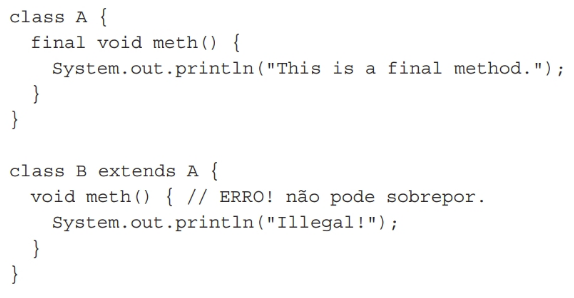
\includegraphics[height=0.5\paperheight]{fig/aula16/final_metodo.png} \\
 \end{center}
\end{frame}
%----------------------------------------------------------------------
\begin{frame}{Palavra chave \textcolor{red}{final}}
  Para impedir que uma classe seja herdada, utilize o modificador 
  \textbf{final} no início de sua declaração.
  \begin{center}
  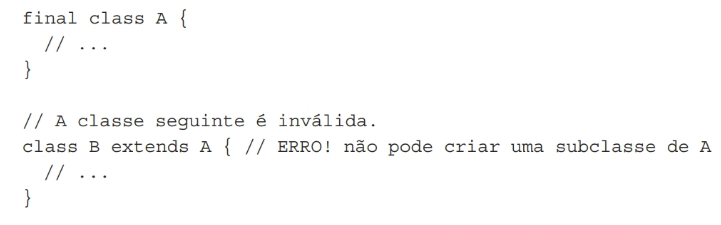
\includegraphics[height=0.35\paperheight]{fig/aula16/final_heranca.png} \\
 \end{center}
\end{frame}
%----------------------------------------------------------------------
\begin{frame}{Palavra chave \textcolor{red}{final}}
  Para impedir que um atributo seja modificado, ou seja, para declarar uma 
  constante utilize o modificador \textbf{final}.
  \begin{center}
  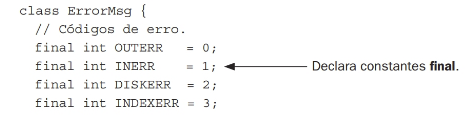
\includegraphics[height=0.25\paperheight]{fig/aula16/final_variavel.png} \\
 \end{center}
\end{frame}
%----------------------------------------------------------------------
\section{Atividade}
\begin{frame}{Atividade}
  \begin{enumerate}
   \item Uma superclasse tem acesso aos membros de uma subclasse? E a subclasse 
pode acessar os membros de uma superclasse? 
  \item Crie uma subclasse de Forma2D chamada Circle. Inclua um método area() 
que calcule a área do círculo e um construtor que use super para inicializar a 
parte referente a Froma2D. 
  \item Como impedir que uma subclasse tenha acesso a um membro de uma 
superclasse? 
%   \item Descreva a finalidade e a aplicação das duas versões de super 
% mostradas neste capítulo. 5.	Dada a hierarquia a seguir: class Alpha { ... 
% class Beta extends Alpha { ... Class Gamma extends Beta { ... Em que ordem os 
% construtores dessas classes concluem sua execução quando um objeto Gamma é 
% instanciado? 6.	Uma referência da superclasse pode referenciar um objeto da 
% subclasse. Expli- que por que isso é importante no âmbito da sobreposição de 
% métodos. 7.	O que é uma classe abstrata? 8.	Como impedir que um 
% método seja sobreposto? E que uma classe seja herdada? 9.	Explique como a 
% herança, a sobreposição de métodos e as classes abstratas são usadas para 
% dar suporte ao polimorfismo. 10.	Que classe é superclasse de todas as 
% outras classes? 11. Uma classe que contém pelo menos um método abstrato deve 
% ser declarada como abstrata. Verdadeiro ou falso? 12.	Que palavra-chave é 
% usada para criar uma constante nomeada?
  \end{enumerate}
\end{frame}
%-----------------------------------------------------------------------
\section{Leitura recomendada}
\begin{frame}{Leitura complementar}
 Para mais informações sobre abstract e final em JAVA, leia:\\
 \begin{columns}
   \begin{column}{0.4\textwidth}
     Java: Como programar\\
     Capítulo 10: \cite{deitel2010java}\\
     \vspace{0.3cm}
      Java para Iniciantes\\
      Capítulo 6
      \cite{schildt2015java}
   \end{column}
   \begin{column}{0.3\textwidth}
    \begin{center}
  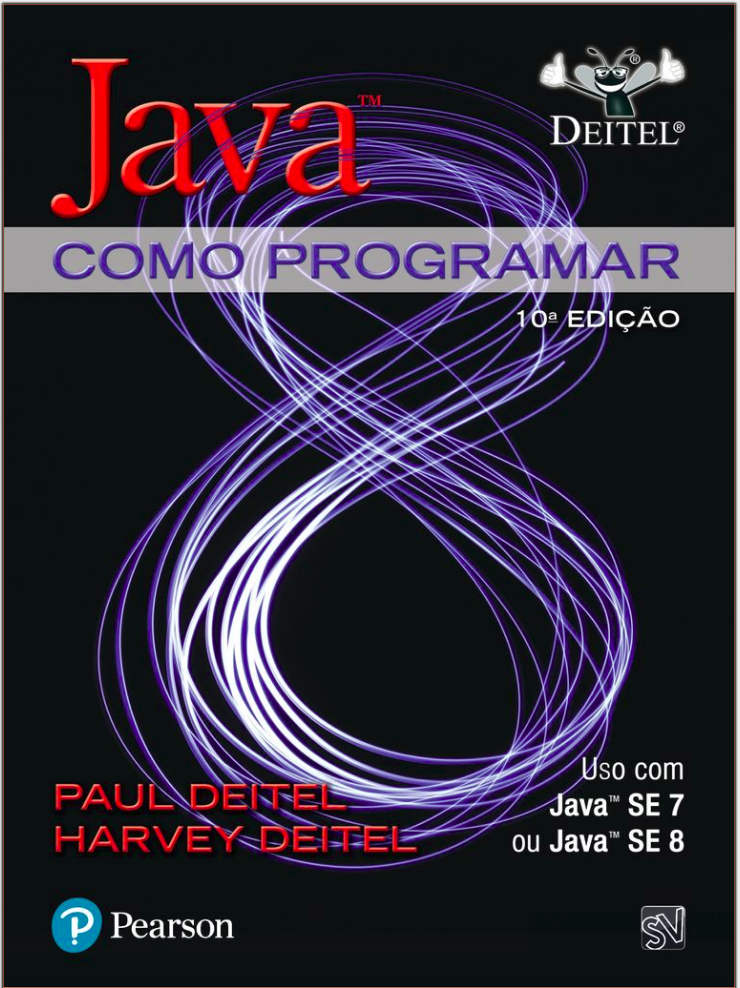
\includegraphics[height=0.5\paperheight]{fig/aula1/deitel2017java.png} \\
 \end{center}
   \end{column}
 \end{columns}
\end{frame}
%----------------------------------------------------------------------
\section{Referências}

\begin{frame}{Referências}%[allowframebreaks]
\small
\begin{center}
\tiny
\bibliographystyle{apalike}
\bibliography{ref_aula_progI}
\end{center}
\end{frame}
\setcounter{framenumber}{\thelastpagemainpart}

\end{document}